\subsection{Single heterologous marker}\label{ex:simplest_het}

\paragraph{Observed and phased alleles} Suppose a single allele is observed at a single marker, indexed by $j$, genotyped in an enrolment infection, $t=0$, and single recurrent infection, $t=1$. Since we detect only one allele per infection we assume there is only one genotype per infection, indexed by $i$, and one way to phase the observed alleles, e.g., 
\begin{equation*}
    \bm{y} = 
    \begin{blockarray}{cl}
    j=1 \\
    \begin{block}{(c)l}
    \{A\} & t=0 \\
    \{T\} & t=1 \\
    \end{block}
    \end{blockarray},
    \hspace{1cm}
    \bm{a} = 
    \begin{blockarray}{cl}
    j=1 \\
    \begin{block}{(c)l}
    A & i=1 \\
    T & i=2. \\
    \end{block}
    \end{blockarray}
\end{equation*}

\paragraph{Relationship graphs}
To compute the posterior probability of the single recurrent state, $s$, being either a relapse, $L$, reinfection, $I$, or recrudescence $C$, we sum over three graphs ($\rg_\RN{1}$, $\rg_\RN{2}, \rg_\RN{3}$) of relationships between parasite genotypes 1 and 2,  
\begin{center}
    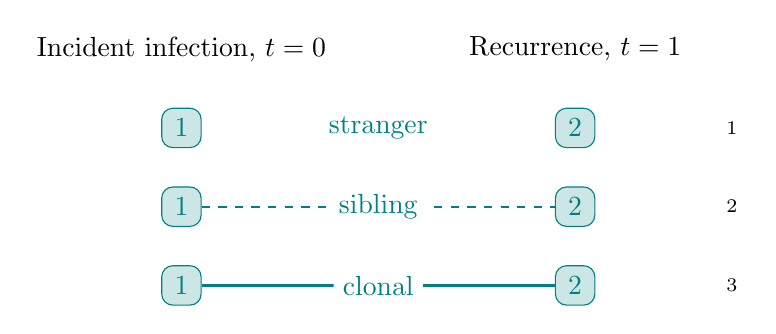
\begin{tikzpicture}

    \tikzstyle{geno} = [draw, rectangle, rounded corners, minimum height=0.5cm, minimum width=0.5cm, color = teal, fill = teal!20]

    % Labels
    \node at (7,0) {$\rg_\RN{1}$};
    \node at (7,-1) {$\rg_\RN{2}$};
    \node at (7,-2) {$\rg_\RN{3}$};
    \node at (0,1) {Incident infection, $t=0$};
    \node at (5,1) {Recurrence, $t=1$};

    % Nodes
    \node[geno] at (0,0) (y1G1) {$1$};
    \node[geno] at (5,0) (y2G1) {$2$};
    \node[geno] at (0,-1) (y1G2) {$1$};
    \node[geno] at (5,-1) (y2G2) {$2$};
    \node[geno] at (0,-2) (y1G3) {$1$};
    \node[geno] at (5,-2) (y2G3) {$2$};

    % Lines
    \path (y1G1) -- (y2G1) node[text = teal, midway]{stranger};
    \draw[geno, dashed, thick] (y1G2) -- (y2G2) node[midway,fill=white]{sibling};
    \draw[geno, thick] (y1G3) -- (y2G3) node[midway,fill=white]{clonal}; 
    \end{tikzpicture}
\end{center}

\paragraph{IBD partitions}
For each relationship graph, we sum over two IBD partitions of genotypes 1 and 2 at the single marker, $\ip_\RN{1} = \{\{1\},\{2\}\}$ and $\ip_\RN{2} = \{\{1,2\}\}$ that correspond to the following two IBD graphs. 
\begin{center}
    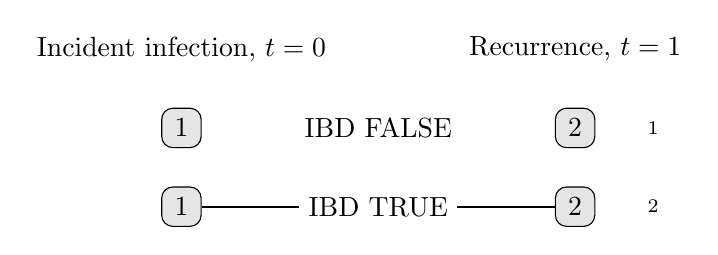
\begin{tikzpicture}

    \tikzstyle{geno} = [draw, rectangle, rounded corners, minimum height=0.5cm, minimum width=0.5cm, fill=gray!20]

    % Labels
    \node at (6,0) {$\ip_\RN{1}$};
    \node at (6,-1) {$\ip_\RN{2}$};
    \node at (0,1) {Incident infection, $t=0$};
    \node at (5,1) {Recurrence, $t=1$};

    % Nodes
    \node[geno] at (0,0) (y1G1) {$1$};
    \node[geno] at (5,0) (y2G1) {$2$};
    \node[geno] at (0,-1) (y1G2) {$1$};
    \node[geno] at (5,-1) (y2G2) {$2$};

    % Lines
    \path (y1G1) -- (y2G1) node[midway]{IBD FALSE};
    \draw[thick] (y1G2) -- (y2G2) node[midway,fill=white]{IBD TRUE};
    
    \end{tikzpicture}
\end{center}

\paragraph{Likelihood} As there is one way to phase the observed alleles and $m=1$, $\mathbb{P}(\bm{y} | s) = \mathbb{P}(\bm{a}|s) = \mathbb{P}(\bm{a}_{\cdot 1}|s)$ where
\small
\begin{equation*}
    \underbrace{
    \begin{blockarray}{lccc}
         & L & I & C \\
        \begin{block}{l(ccc)}
        \bm{a} & \sfrac{1}{2}f(A)f(T) & f(A)f(T) & 0  \\
        \end{block}
        \end{blockarray}
    }_{\mathclap{\mathbb{P}(\bm{a}|s)\forall s\in\{L,I,C\}}}
    =
    \underbrace{
    \begin{blockarray}{ccl}
        \ip_\RN{1} & \ip_\RN{2} \\
        \begin{block}{(cc)l}
          f(A)f(T) & 0 & \bm{a}_{\cdot 1} \\
        \end{block}
        \end{blockarray}
    }_{\mathclap{\mathbb{P}(\bm{a}_{\cdot j}|\ip)\forall\bm{a}_{\cdot j}\in\bm{a}, \ip\in\IP}}
    \times\;
    \underbrace{
    \begin{blockarray}{cccl}
        \rg_\RN{1}, & \rg_\RN{2}, & \rg_\RN{3} & \\
        \begin{block}{(ccc)l}
         1 & \sfrac{1}{2} & 0 & \ip_\RN{1} \\
         0 & \sfrac{1}{2} & 1 & \ip_\RN{2} \\
        \end{block}
        \end{blockarray}
    }_{\mathclap{\mathbb{P}(\ip | \rg)\forall \ip \in \IP, \rg\in\RG}}
    \times\;
    \underbrace{
    \begin{blockarray}{cccc}
        L & I & C & \\
        \begin{block}{(ccc)l}
          \sfrac{1}{3} & 1 & 0 & \rg_\RN{1} \\
          \sfrac{1}{3} & 0 & 0 & \rg_\RN{2} \\
          \sfrac{1}{3} & 0 & 1 & \rg_\RN{3} \\
        \end{block}
        \end{blockarray},
    }_{\mathclap{\mathbb{P}(\rg|s) \forall \rg\in\RG, s\in\{L,I,C\}}}
\end{equation*}
\normalsize
%
and
\begin{align*}
\mathbb{P}(\bm{a}_{\cdot 1} | \ip_\RN{1}) 
&= \mathbb{P}(\{A\} | \{1\}) \times \mathbb{P}(\{T\}|\{2\})
= f(A)f(T).\\
\mathbb{P}(\bm{a}_{\cdot 1} | \ip_\RN{2}) 
&= \mathbb{P}(\{A,T\} | \{1, 2\})
= 0 \text{ because }|\{A,T\}| \neq 1. 
\end{align*}


\paragraph{Posterior} For a uniform prior on $s$, $\mathbb{P}(y) = \sfrac{1}{2}f(A)f(T)$, such that $\mathbb{P}(s = L|\bm{y}) = \sfrac{1}{3}$, $\mathbb{P}(s = I|\bm{y}) = \sfrac{2}{3}$ and $\mathbb{P}(s = C|\bm{y}) = 0$. \\

%=========================================================
\subsection{Single homologous marker} \label{ex:simplest_hom}
For $\bm{y} = (\{A\}, \{A\})^{T}$ and a uniform prior on s, $\mathbb{P}(y) = \sfrac{1}{2}f(A)^2 + \sfrac{1}{2}f(A)$, such that $\mathbb{P}(s = L|\bm{y}) = \sfrac{1}{3}$, $\mathbb{P}(s = I|\bm{y}) = \sfrac{2}{3}f(A)(f(A)+1)^{-1}$ and $\mathbb{P}(s = C|\bm{y}) = \sfrac{2}{3}(f(A)+1)^{-1}$ following
\small
\begin{equation*}
    \underbrace{
    \begin{blockarray}{lccc}
         & L & I & C \\
        \begin{block}{l(ccc)}
        \bm{a} & \sfrac{1}{2}f(A)^2 + \sfrac{1}{2}f(A) & f(A)^2 & f(A)  \\
        \end{block}
        \end{blockarray}
    }_{\mathclap{\mathbb{P}(\bm{a}|s)\forall s\in\{L,I,C\}}}
    =
    \underbrace{
    \begin{blockarray}{ccl}
        \ip_\RN{1} & \ip_\RN{2} \\
        \begin{block}{(cc)l}
          f(A)^2 & f(A) & \bm{a}_{\cdot 1} \\
        \end{block}
        \end{blockarray}
    }_{\mathclap{\mathbb{P}(\bm{a}_{\cdot j}|\ip)\forall \bm{a}_{\cdot j}\in\bm{a}, \ip\in\IP}}
    \times\;
    \underbrace{
    \begin{blockarray}{cccl}
        \rg_\RN{1}, & \rg_\RN{2}, & \rg_\RN{3} & \\
        \begin{block}{(ccc)l}
         1 & \sfrac{1}{2} & 0 & \ip_\RN{1} \\
         0 & \sfrac{1}{2} & 1 & \ip_\RN{2} \\
        \end{block}
        \end{blockarray}
    }_{\mathclap{\mathbb{P}(\ip|\rg)\forall \ip\in\IP, \rg\in\RG}}
    \times\;
    \underbrace{
    \begin{blockarray}{cccc}
        L & I & C & \\
        \begin{block}{(ccc)l}
          \sfrac{1}{3} & 1 & 0 & \rg_\RN{1} \\
          \sfrac{1}{3} & 0 & 0 & \rg_\RN{2} \\
          \sfrac{1}{3} & 0 & 1 & \rg_\RN{3} \\
        \end{block}
        \end{blockarray}.
    }_{\mathclap{\mathbb{P}(\rg|s) \forall \rg\in\RG, s\in\{L,I,C\}}}
\end{equation*}
\normalsize